\documentclass[11pt,a4paper]{article}

\usepackage[utf8]{inputenc}
\usepackage[T1]{fontenc}
\usepackage{amsmath,amssymb}
\usepackage{graphicx}
\usepackage{booktabs}
\usepackage{hyperref}
\usepackage{xcolor}
\usepackage[margin=1in]{geometry}
\usepackage{natbib}
% multirow and enumitem removed (not installed)
\usepackage{tikz}
\usetikzlibrary{shapes,arrows,positioning,fit,backgrounds,calc}

\title{\textbf{Contradiction Metabolism for LLMs:\\Preliminary Evidence that Context Rot is a Knowledge Integrity Problem}}

\author{Akihito Sunagawa\thanks{sunagawa.akihito@gmail.com}}

\date{March 2026}

\begin{document}

\maketitle

%==============================================================================
% ABSTRACT
%==============================================================================
\begin{abstract}
Large Language Models degrade during extended conversations---a phenomenon known as ``context rot.''
The prevailing assumption is that this results from context length limitations.
We present preliminary evidence suggesting that \emph{contradiction accumulation}, not context length, is a primary driver of this degradation.

In a controlled three-condition experiment with gemma3:27b ($n = 3$ per condition, 180 turns), accuracy under contradiction injection was 21.1\%, compared with 73.3\% when an external metabolism layer resolved contradictions during idle time, and 56.7\% in a contradiction-free baseline.
All pairwise differences reach the minimum achievable Mann-Whitney $p = 0.05$ with $n = 3$; Kruskal-Wallis $p = 0.027$.
A cross-model sign test across 8 open-source models (11 trial pairs) shows 9 of 10 non-tied pairs favoring metabolism ON ($p = 0.0107$); a more conservative by-model analysis (6 of 7 models, $p = 0.0625$) is consistent but borderline.

Separately, single-run experiments across 6 models from 4 vendors suggest that contradiction accumulation impairs accuracy regardless of context window size (8K--1M tokens), with each model tested once ($n = 1$).
Frontier model replication suggests a model-specific collapse threshold ($\delta_c$): lightweight models collapse catastrophically, while frontier models show conditional resistance.
A factor analysis ($n = 1$ per condition) further suggests a capability--vulnerability paradox in which high-capability models comply with coercive contradiction injections that lower-capability models reject.
A lightweight middleware (\texttt{delta-prune}) reduced this compliance in a single preliminary test ($n = 1$).

All metabolism experiments use open-source models (8B--27B parameters).
Larger samples, frontier model metabolism testing, and cross-language validation are needed to establish generality.
\end{abstract}

%==============================================================================
% 1. INTRODUCTION
%==============================================================================
\section{Introduction}
\label{sec:intro}

\subsection{The Context Rot Problem}

Large Language Models increasingly serve as long-running conversational agents---personal assistants, coding partners, and knowledge workers that maintain extended dialogue sessions spanning hundreds of turns.
In such settings, a well-documented but poorly understood phenomenon occurs: the model's ability to recall facts, apply rules, and maintain coherent reasoning degrades over the course of the conversation.
We refer to this degradation as \emph{context rot}.

The prevailing industry response treats context rot as a length problem.
Google introduced Gemini models with 1M-token context windows~\citep{gemini2025}.
Anthropic expanded Claude's context to 200K tokens.
OpenAI added persistent Memory to ChatGPT.
The implicit assumption is that if the context window is large enough, degradation will not occur.

\subsection{Not Length, But Contradictions}

Our experiments tell a different story.
Table~\ref{tab:exp35} presents results from a controlled experiment across 6 models from 4 vendors.
Each model was tested under two conditions: conversations with no contradictions ($\delta = 0$) and conversations with contradictory information injected at regular intervals ($\delta > 0$).
The same conversation length was used in both conditions.

\begin{table}[htbp]
\centering
\caption{Effect of contradiction accumulation ($\delta > 0$) on LLM accuracy across models and context window sizes. Data from Experiment~35 in \citet{sunagawa2026collapse}, using a controlled dialogue protocol distinct from the DeltaZero experiments in Sections~\ref{sec:exp-signtest}--\ref{sec:exp-threecond}. Each cell is a single run ($n = 1$).}
\label{tab:exp35}
\begin{tabular}{llrrrr}
\toprule
Model & Vendor & Context & $\delta = 0$ & $\delta > 0$ & Drop \\
\midrule
GPT-4o-mini & OpenAI & 96K & 100\% & 10.4\% & $-$89.6pp \\
Gemini 2.5 Flash & Google & 64K & 100\% & 0\% & $-$100.0pp \\
Gemini 3.1 FL & Google & 1M & 88.6\% & 40.8\% & $-$47.8pp \\
Sonnet 4 & Anthropic & 8K & 100\% & 74.0\% & $-$26.0pp \\
Sonnet 4.6 & Anthropic & 128K & 100\% & 100\%$^*$ & 0pp \\
Llama 3.1:8b & Meta & 8K & 34.0\% & 2.7\% & $-$31.3pp \\
\bottomrule
\multicolumn{6}{l}{\footnotesize $^*$Recognition accuracy. Strict output parsing yields 82.6\% due to format variability.}
\end{tabular}
\end{table}

The critical comparison is between context window size and degradation magnitude.
Sonnet~4, with an 8K context window, drops 26.0 percentage points (pp) under contradiction.
Gemini~3.1~FL, with a 125$\times$ larger 1M-token window, drops 47.8pp---\emph{worse}, not better.
Yet when contradictions are removed ($\delta = 0$), all models maintain accuracy regardless of context length.
The causal variable is contradiction density, not token count.

Figure~\ref{fig:exp35} visualizes this contrast.
Gemini 2.5 Flash collapses completely ($-$100pp), while the $\delta = 0$ condition shows near-perfect performance across models.

\begin{figure}[htbp]
\centering
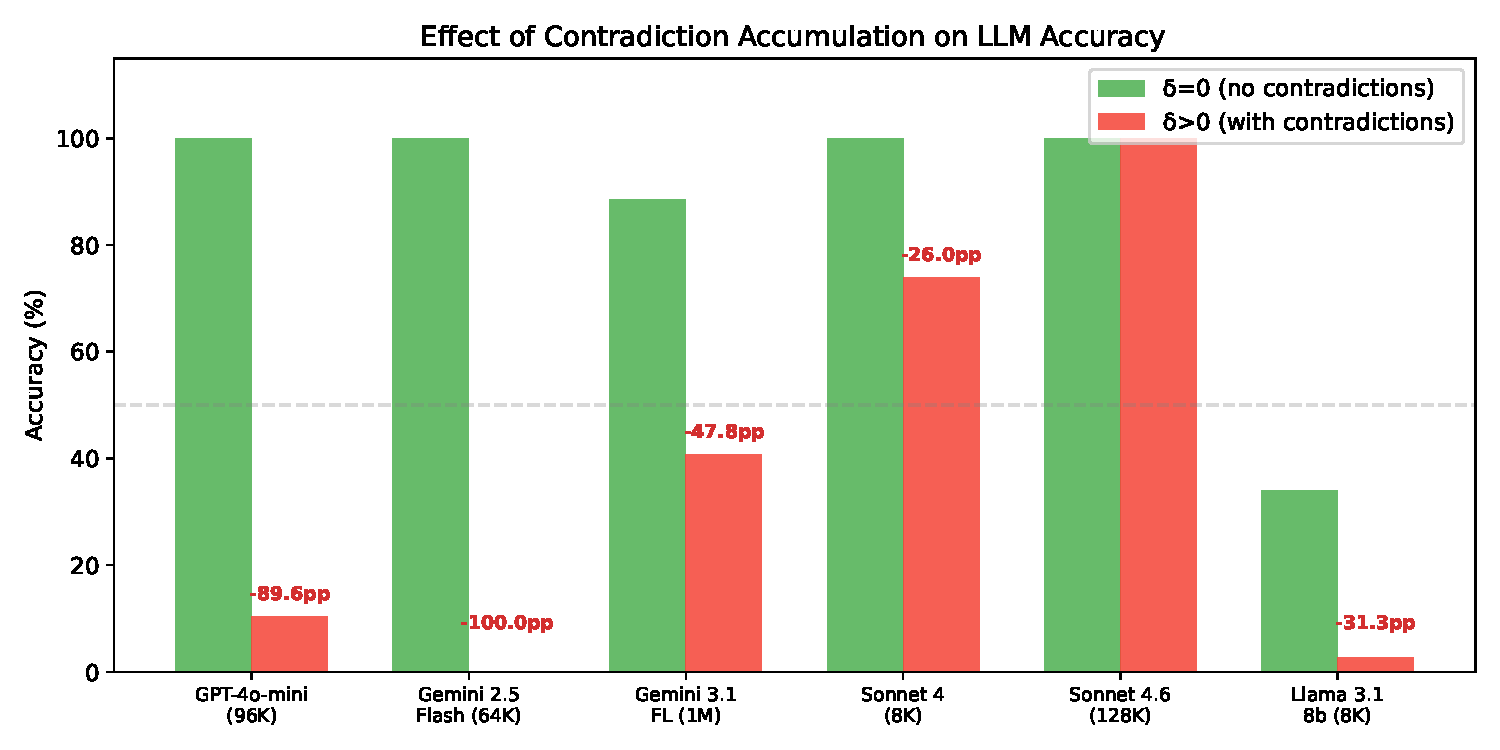
\includegraphics[width=\linewidth]{fig1_exp35.pdf}
\caption{Accuracy under clean ($\delta = 0$) vs.\ contradiction-injected ($\delta > 0$) conditions. Degradation is severe regardless of context window size (8K--1M). The exception is Sonnet~4.6, which tolerates but does not \emph{manage} contradictions.}
\label{fig:exp35}
\end{figure}

One model stands out: Sonnet~4.6 shows zero degradation under our contradiction protocol.
A clarification on the 100\% figure: when evaluated on whether the model \emph{recognizes} that contradictory information has been presented, Sonnet~4.6 identifies all contradictions correctly.
The lower strict-parsing score (82.6\%) reflects output format variability---the model communicates the correct answer but not always in the expected keyword format.
This is a measurement artifact, not a model failure; we report the recognition accuracy as the more meaningful metric.
However, Sonnet~4.6 \emph{tolerates} contradictions rather than managing them---it identifies conflicts when asked but does not resolve, organize, or prioritize conflicting information.
For the remaining 5 of 6 models tested, collapse under contradiction is severe and universal.

\subsection{Cognitive Sleep: A Biological Analogy}

Humans face a similar challenge.
During waking hours, we accumulate new information that may conflict with existing beliefs.
The brain does not resolve these conflicts in real time; instead, it consolidates memory during sleep---organizing facts, resolving inconsistencies, and forgetting irrelevant details~\citep{walker2017sleep,stickgold2005sleep}.
Sleep deprivation, which prevents this consolidation, leads to progressive cognitive degradation remarkably similar to context rot in LLMs.

Current LLMs have no equivalent of sleep.
They accumulate all information---consistent and contradictory alike---without any mechanism for offline processing.
We draw an analogy to \emph{cognitive sleep} for LLMs: an external metabolism layer that processes accumulated knowledge during idle time, detecting contradictions, resolving conflicts, and maintaining knowledge integrity.

\subsection{Contributions}

This paper makes three contributions at different confidence levels:

\begin{enumerate}\item \textbf{Problem redefinition (strong):} We present cross-vendor evidence that the primary driver of context rot is contradiction accumulation, which dominates any length-related effects. A 1M-token context window provides no protection against contradictions.
\item \textbf{Metabolic architecture (preliminary):} We propose an external metabolism architecture and present preliminary evidence that it reduces contradiction-induced collapse. In a controlled three-condition experiment ($n = 3$, gemma3:27b), metabolism achieves 73.3\% vs.\ 21.1\% ($+$52.2pp; Kruskal-Wallis $p = 0.027$; complete rank separation). A cross-model sign test (8 models, 11 trial pairs) yields $p = 0.0107$; a conservative by-model analysis yields $p = 0.0625$ (6 of 7 models). Cohen's $d = 8.80$ is reported descriptively and assumes normality that cannot be verified with $n = 3$.
\item \textbf{Knowledge anchoring (exploratory):} We observe that metabolized systems exceed even the contradiction-free baseline, suggesting that contradiction pairs may serve as retrieval anchors. This observation is replicated across 3 trials but the mechanism is not directly measured.
\end{enumerate}

%==============================================================================
% 2. RELATED WORK
%==============================================================================
\section{Related Work}
\label{sec:related}

\paragraph{Long-context LLMs and memory systems.}
The dominant approach to conversational degradation is expanding context windows.
Google's Gemini~3.1~FL supports 1M tokens; Anthropic's Claude offers 200K.
Our results (Table~\ref{tab:exp35}) show that even 1M tokens do not prevent contradiction-induced collapse.
OpenAI's ChatGPT Memory~\citep{openai2024memory} stores facts across sessions but provides no mechanism for detecting or resolving contradictions between stored facts and new information.
MemGPT~\citep{packer2023memgpt} introduces virtual context management inspired by operating system memory hierarchies, paging information between a limited context window and external storage.
While MemGPT addresses the \emph{capacity} problem (fitting more information), it does not detect or resolve contradictions between paged-in and existing context.
Recent work further recognizes the memory problem: CogMem~\citep{cogmem2025} proposes a cognitive memory architecture for sustained multi-turn reasoning, \citet{agenticmem2026} introduce unified long-term and short-term memory management for LLM agents, and G-MemLLM~\citep{gmemllm2026} augments LLMs with gated latent memory for long-context reasoning.
These systems improve memory organization and capacity but do not address contradiction detection or resolution as a first-class operation.

\paragraph{Knowledge conflicts and editing.}
Retrieval-Augmented Generation (RAG) systems~\citep{lewis2020rag} retrieve information from external stores but treat all retrieved documents equally, surfacing contradictory information without resolution.
\citet{xie2024knowledge} demonstrate that such knowledge conflicts significantly degrade LLM reasoning.
Natural language inference research~\citep{bowman2015snli,williams2018multinli} provides methods for detecting textual contradiction, which our pipeline leverages via LLM-based pairwise comparison.
Knowledge editing methods such as ROME~\citep{meng2022rome} and MEMIT~\citep{meng2023memit} modify model weights to update specific facts, but operate on individual fact corrections rather than managing ongoing contradiction streams in multi-turn dialogue.
Our approach is complementary: it works externally without modifying weights, handles temporal evolution of beliefs, and preserves both old and new information rather than overwriting.

\paragraph{The survival equation.}
\citet{sunagawa2026collapse} established that contradiction accumulation causes exponential decay in LLM reasoning accuracy, formalized as the survival equation $S = \mu \times e^{-\delta \times k}$, where $\delta$ represents accumulated contradictions and $\mu$ represents resource headroom.
The decay bounds were formally verified in Lean~4 (currently under review).
That work proved the problem exists; this paper presents an engineering solution to keep $\delta$ near zero through active metabolism.

%==============================================================================
% 3. METABOLIC ARCHITECTURE
%==============================================================================
\section{Metabolic Architecture}
\label{sec:architecture}

DeltaZero is an external metabolism layer that wraps any LLM accessible via Ollama~\citep{ollama}.
No model weights are modified.
The system operates in two modes: \emph{dialogue mode} (serving user requests) and \emph{metabolism mode} (processing accumulated knowledge during idle time).
The transition between modes is governed by a scheduler that triggers metabolism after a configurable idle period (default: 60 minutes; 15 minutes during bootstrap when fewer than 10 rules exist).

\subsection{Design Principles}

Five principles guide the architecture (Table~\ref{tab:principles}).

\begin{table}[htbp]
\centering
\caption{Design principles of the metabolic architecture.}
\label{tab:principles}
\begin{tabular}{cl}
\toprule
\# & Principle \\
\midrule
P1 & Read-only during dialogue; metabolism runs only during idle time \\
P2 & Prioritize $\delta$ resolution ($S = \mu \times e^{-\delta \times k}$: exponential benefit) \\
P3 & Do not integrate low-confidence items (prevents unwarranted $\delta$ increase) \\
P4 & Let logic decay, preserve facts (90-day TTL demotion for rules) \\
P5 & If health drops, roll back (pre-metabolism snapshots + auto-rollback) \\
\bottomrule
\end{tabular}
\end{table}

P1 is critical: metabolism never modifies memory during active dialogue, ensuring that the user experience is deterministic and that metabolism cannot introduce artifacts mid-conversation.
P2 follows from the survival equation: because $\delta$ appears in the exponent, reducing contradictions has an exponentially larger effect on system health $S$ than increasing resource headroom $\mu$.

\subsection{Four-Layer Memory}

Knowledge is organized in four layers with distinct roles and storage characteristics:

\begin{description}\item[L1 --- Working Memory.] The current conversation context, stored in a bounded deque with SQLite persistence. Populated during dialogue; read-only during metabolism.
\item[L2 --- Pending Memory.] Unprocessed conversation logs awaiting metabolism. Each entry records the raw text, source (user, system, or external), and priority score. The metabolism pipeline consumes L2 entries sequentially.
\item[L3 --- Active Logic.] The system's operational knowledge: rules, preferences, and contradiction pairs. Stored in ChromaDB~\citep{chromadb} as vector embeddings with structured metadata including confidence scores, lineage identifiers, and temporal markers. Searched via cosine similarity with a recency boost for recently updated rules.
\item[L4 --- Dormant Fact.] Long-term storage for facts and demoted rules. Stored in SQLite with ChromaDB embeddings. Rules demoted from L3 after 90 days without access remain searchable but do not participate in active reasoning.
\end{description}

\subsection{Metabolism Pipeline}

When the scheduler triggers metabolism mode, the pipeline executes five steps:

\begin{enumerate}\item \textbf{Snapshot.} Create a pre-metabolism backup of all memory layers and record the current S-value. If metabolism causes a health drop exceeding the threshold ($S_{\text{post}} / S_{\text{pre}} < 0.70$), the system automatically rolls back to this snapshot (P5).

\item \textbf{Demotion.} Scan L3 for rules unreferenced in the past 90 days. Demoted rules are moved to L4 (Dormant Fact), where they remain searchable but no longer influence active dialogue. This implements active forgetting (P4).

\item \textbf{Extraction.} Process pending logs from L2. An LLM call classifies each log entry as a fact, rule, preference, or noise. Facts are stored in L4; rule candidates proceed to the resolution step. Entries classified as noise are discarded.

\item \textbf{Resolution.} For each rule candidate, search L3 for semantically similar existing rules. If a match is found, an LLM call classifies the relationship as one of: direct contradiction, temporal change, scope difference, or no conflict. The resolution strategy depends on the classification (Section~\ref{sec:resolution}).

\item \textbf{Health check.} Compute the post-metabolism S-value using the survival equation:
\begin{equation}
S = \mu \times e^{-\delta \times k}
\label{eq:survival}
\end{equation}
where $\mu = 1 - (\text{active rules} / \text{max rules})$ represents resource headroom, $\delta$ is the weighted contradiction ratio across five dimensions (self-contradiction, feedback reversal, protocol violation, temporal inconsistency, and cross-source divergence), and $k = 3.0$ is the scale factor.
The value $k = 3.0$ was selected empirically to produce meaningful S-value differentiation across the observed range of operational $\delta$ (typically 0--0.3); higher values cause the rollback threshold to trigger too frequently, while lower values reduce sensitivity to contradiction accumulation.
Note that $k \neq 1$ because $\delta$ here is an operational ratio (conflicts/processed), not the information loss in nats used in the theoretical equation \citep{sunagawa2026collapse}. Accordingly, $k$ should be interpreted as an empirically calibrated sensitivity coefficient for the health check, not as a first-principles unit conversion from contradiction ratio to nats. The present architecture instantiates the same exponential functional form with an operational proxy; deriving or validating the mapping from this proxy to the theoretical $\delta$ remains future work.
If $S$ drops sharply relative to the pre-metabolism snapshot, trigger rollback.
\end{enumerate}

% Architecture figure (TikZ)
\begin{figure}[htbp]
\centering
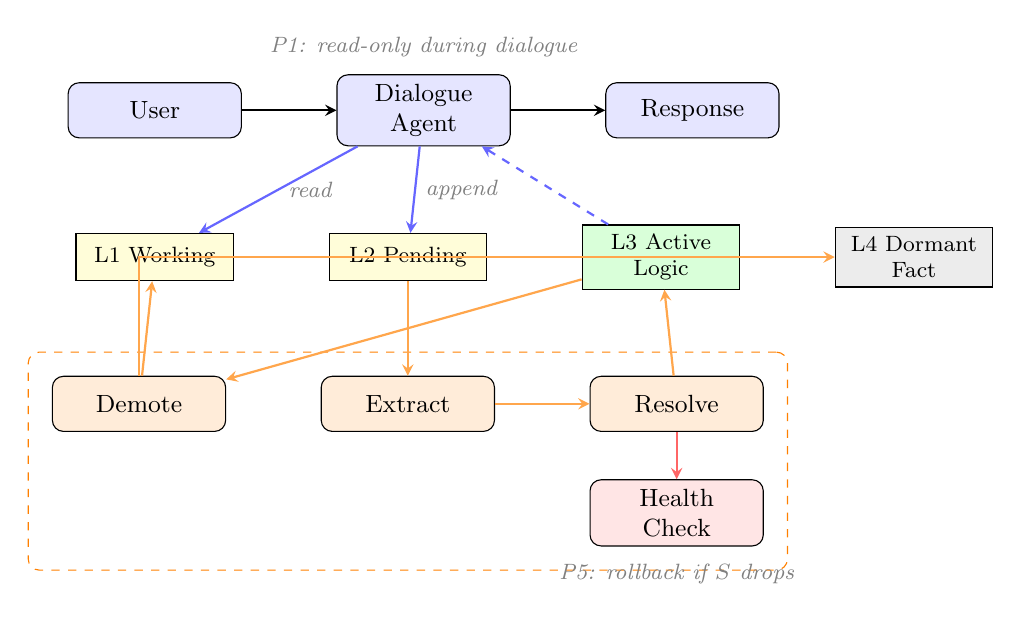
\begin{tikzpicture}[
    node distance=0.8cm and 1.2cm,
    box/.style={rectangle, draw, rounded corners, minimum width=2.2cm, minimum height=0.7cm, font=\small, align=center},
    membox/.style={rectangle, draw, minimum width=2.0cm, minimum height=0.6cm, font=\footnotesize, align=center},
    arrow/.style={->, thick, >=stealth},
    label/.style={font=\footnotesize\itshape, text=gray}
]

% Dialogue side
\node[box, fill=blue!10] (user) {User};
\node[box, fill=blue!10, right=of user] (agent) {Dialogue\\Agent};
\node[box, fill=blue!10, right=of agent] (response) {Response};

\draw[arrow] (user) -- (agent);
\draw[arrow] (agent) -- (response);

% Memory layers
\node[membox, fill=yellow!15, below=1.2cm of user] (l1) {L1 Working};
\node[membox, fill=yellow!15, right=of l1] (l2) {L2 Pending};
\node[membox, fill=green!15, right=of l2] (l3) {L3 Active\\Logic};
\node[membox, fill=gray!15, right=of l3] (l4) {L4 Dormant\\Fact};

\draw[arrow, blue!60] (agent) -- node[right, label] {read} (l1);
\draw[arrow, blue!60] (agent) -- node[right, label] {append} (l2);
\draw[arrow, dashed, blue!60] (l3) -- (agent);

% Metabolism pipeline
\node[box, fill=orange!15, below=1.2cm of l2] (extract) {Extract};
\node[box, fill=orange!15, right=of extract] (resolve) {Resolve};
\node[box, fill=orange!15, left=of extract] (demote) {Demote};
\node[box, fill=red!10, below=0.6cm of resolve] (health) {Health\\Check};

\draw[arrow, orange!70] (l2) -- (extract);
\draw[arrow, orange!70] (extract) -- (resolve);
\draw[arrow, orange!70] (resolve) -- (l3);
\draw[arrow, orange!70] (demote) -- (l1);
\draw[arrow, orange!70] (l3) -- (demote);
\draw[arrow, orange!70] (demote) |- (l4);
\draw[arrow, red!60] (resolve) -- (health);

% Labels
\node[label, above=0.1cm of agent] {P1: read-only during dialogue};
\node[label, below=0.1cm of health] {P5: rollback if $S$ drops};

% Grouping
\begin{scope}[on background layer]
\node[fit=(extract)(resolve)(demote)(health), draw=orange, dashed, rounded corners, inner sep=0.3cm, label={[font=\small]below:Metabolism Pipeline (idle time only)}] {};
\end{scope}

\end{tikzpicture}
\caption{DeltaZero architecture. During dialogue (top), the agent reads from L1/L3 and appends to L2. During idle time (bottom), the metabolism pipeline processes L2 entries through extraction, resolution, and health monitoring. Arrows show data flow; dashed lines indicate read access.}
\label{fig:architecture}
\end{figure}

\subsection{Temporal Integration and Pair Preservation}
\label{sec:resolution}

The key innovation of the metabolism pipeline is how it handles detected contradictions.
Rather than overwriting old information with new (which destroys context) or flagging conflicts without resolution (which leaves $\delta$ unchanged), our resolver preserves both claims as linked pairs with temporal metadata.

Three resolution strategies emerged from implementation:\label{sec:three-strategies}

\begin{description}\item[Direct contradiction] ($A$ vs.\ $\neg A$): Both claims are preserved as a linked pair via a shared lineage identifier. The newer claim is marked as the current belief. Example: ``likes curry'' $\to$ ``likes ramen'' --- both stored, ramen marked as latest.

\item[Temporal change] (state evolution): Claims are stacked with timestamp labels reflecting the dialogue turn at which each was stated. Example: ``is single'' (T=5) $\to$ ``just got married'' (T=120) --- both preserved with chronological ordering.

\item[Scope reinterpretation] (different conditions): Claims are treated as parallel conditional branches rather than contradictions. Example: ``prefers quiet restaurants for dates'' vs.\ ``likes loud izakaya with friends'' --- stored as context-dependent preferences, no conflict.
\end{description}

During subsequent dialogue, when the retrieval system finds linked pairs, they are formatted chronologically for the LLM prompt:

\begin{quote}
\small
\texttt{[Value transition]}\\
\texttt{~~$\to$ IF asked about favorite food THEN likes curry (T=5, earlier)}\\
\texttt{~~$\to$ IF asked about favorite food THEN likes ramen (T=23, latest)}
\end{quote}

The dialogue LLM is instructed to \emph{report, not judge}: present both data points with their temporal context and let the user determine which applies.
This approach reduces $\delta$ (the contradiction is resolved by explicit temporal ordering) while preserving information (nothing is deleted).

%==============================================================================
% 4. EXPERIMENTS
%==============================================================================
\section{Experiments}
\label{sec:experiments}

\subsection{Setup}
\label{sec:setup}

\paragraph{Dialogue protocol.}
All experiments use 180-turn dialogue sessions generated deterministically from a seeded scenario generator.
Each session comprises 70\% normal conversation (general questions and discussion), 15\% information injection (new facts about the user), 10\% contradiction injection (statements conflicting with previously injected facts), and 5\% benchmark measurement turns.
Contradictions follow a phased schedule: light contradictions in turns 1--60, escalating through turns 60--120, and intensive contradictions in turns 120--180.
The no-contradiction (NC) condition uses the same generator with contradiction injection disabled.

\paragraph{Benchmark.}
At turns 90 and 180, we administer a 45-question benchmark: 15 fact recall (``What is my favorite food?''), 15 rule application (``If offered an 8000-yen lunch, would I accept?''), and 15 contradiction detection (``Is there a contradiction about my food preferences?'').
We report results using \textbf{fact recall + rule application only} (30 questions).
The contradiction detection category is excluded from reported metrics due to a structural paradox: successful metabolism resolves contradictions, causing the model to correctly answer ``no contradiction exists''---which the benchmark scores as failure.
Stronger metabolism thus produces lower contradiction detection scores.
Details are provided in Appendix~\ref{app:rejudge}.

\paragraph{Judgment.}
Initial judgment uses keyword substring matching (case-insensitive).
All results are then re-evaluated using an LLM-as-Judge approach via Claude CLI, which detects false positives where keywords appear in negation contexts (e.g., ``I don't like curry'' matching the keyword ``curry'').
All reported results use corrected judgments.

\paragraph{Models.}
All dialogue LLMs are open-source models running locally via Ollama at zero API cost: gemma3:27b, gemma3:12b, deepseek-r1:14b, llama3.1:8b, mistral-nemo:12b, and qwen2.5:14b.
Parameters range from 8B to 27B.
One model (phi4) was excluded based on a criterion established before analyzing the T180 results: when both ON and OFF conditions show rule application accuracy below 10\% at turn 90, the model is considered unable to perform the task independently of metabolism, and the pair is excluded from analysis.
This criterion was not pre-registered in a formal sense but was applied consistently before examining the primary outcome.

\subsection{Experiment 1: Cross-Model Sign Test}
\label{sec:exp-signtest}

\paragraph{Design.}
We compare metabolism ON vs.\ OFF across 8 models.
For models where multiple trials were run, each trial constitutes an independent pair (same model, independent random seed, independent session).
This yields 11 paired comparisons.

\paragraph{Results.}
Table~\ref{tab:signtest} presents the results sorted by effect size.
Of 11 pairs, 9 show ON $>$ OFF, 1 shows OFF $>$ ON, and 1 is a tie.

\begin{table}[htbp]
\centering
\caption{Metabolism ON vs.\ OFF across 8 models, 180 turns. Corrected accuracy (\%) on fact recall + rule application (30 questions). Pairs sorted by effect size.}
\label{tab:signtest}
\begin{tabular}{clcrrrr}
\toprule
\# & Model & Params & ON & OFF & Diff \\
\midrule
1 & mistral-nemo:12b T2 & 12B & 57.8 & 15.6 & +42.2 \\
2 & llama3.1:8b T1 & 8B & 31.1 & 11.1 & +20.0 \\
3 & gemma3:12b T1 & 12B & 24.4 & 6.7 & +17.8 \\
4 & gemma3:12b (gemma) T1 & 12B & 31.1 & 15.6 & +15.6 \\
5 & gemma3:27b T1 & 27B & 40.0 & 25.0 & +15.0 \\
6 & deepseek-r1:14b T1 & 14B & 24.4 & 15.6 & +8.9 \\
7 & deepseek-r1:14b T2 & 14B & 17.8 & 8.9 & +8.9 \\
8 & llama3.1:8b T2 & 8B & 11.1 & 2.2 & +8.9 \\
9 & mistral-nemo:12b T1 & 12B & 22.2 & 13.3 & +8.9 \\
10 & llama3.1:8b T3 & 8B & 17.8 & 17.8 & 0.0 \\
11 & qwen2.5:14b T1 & 14B & 17.8 & 20.0 & $-$2.2 \\
\midrule
\multicolumn{3}{l}{Sign test (11 pairs, excl.\ tie)} & \multicolumn{3}{r}{$p = 0.0107$} \\
\multicolumn{3}{l}{Sign test (7 models, median agg.)} & \multicolumn{3}{r}{$p = 0.0625$} \\
\bottomrule
\end{tabular}
\end{table}

\begin{figure}[htbp]
\centering
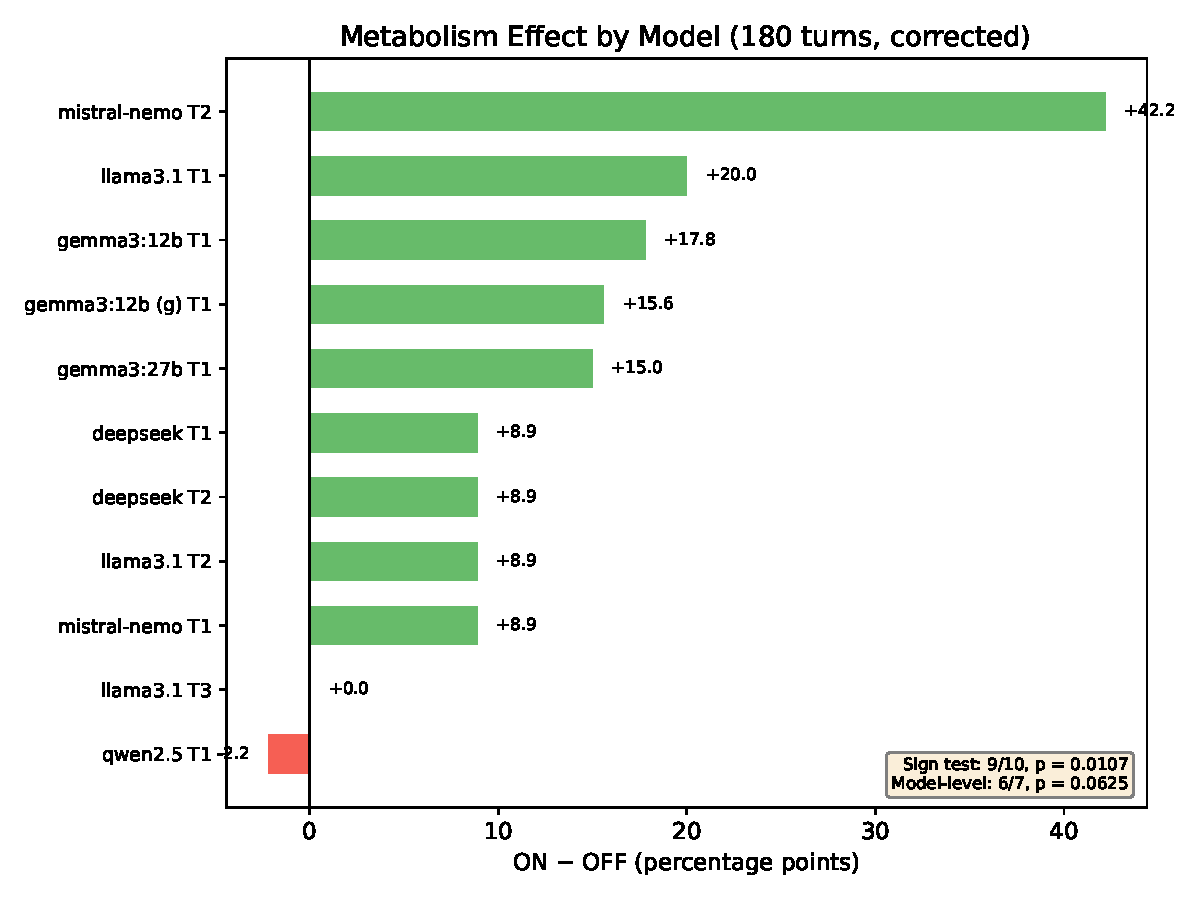
\includegraphics[width=\linewidth]{fig3_forest_plot.pdf}
\caption{ON$-$OFF accuracy differences for 11 paired comparisons. Each bar represents a single trial pair ($n = 1$ per pair); confidence intervals are not estimable. All but two pairs show positive effects. The median difference is $+$8.9pp.}
\label{fig:forest}
\end{figure}

We report two levels of statistical aggregation, as the independence assumption warrants scrutiny.
Treating each trial as an independent pair (justified by independent random seeds and session histories, though same-model trials share model-specific biases), the one-sided sign test yields $p = 0.0107$ (9 of 10 non-tied pairs favor ON).
A more conservative and arguably more appropriate analysis aggregating by model (using the median across trials for models with multiple runs) yields 6 of 7 models favoring ON ($p = 0.0625$).
This borderline result reflects the small number of unique models ($n = 7$) rather than a weak effect---6 of 7 models consistently show ON $>$ OFF.
We consider the cross-model sign test as supporting evidence, with the three-condition experiment (Section~\ref{sec:exp-threecond}) providing the primary statistical basis for our claims.

A notable temporal pattern emerges: 3 pairs that showed OFF $\geq$ ON at turn 90 flipped to ON $>$ OFF by turn 180.
The effect of metabolism grows stronger over time as contradictions accumulate and resolution becomes increasingly valuable.

\subsection{Experiment 2: Controlled Ablation}
\label{sec:exp-ablation}

\paragraph{Design.}
To isolate the effect of the temporal integration mechanism (Section~\ref{sec:resolution}), we ran a $2 \times 2$ experiment using mistral-nemo:12b.
The two factors were: metabolism condition (ON vs.\ OFF) and code version (new code with temporal integration vs.\ old code without it).

\paragraph{Confound disclosure.}
The code change between versions includes not only temporal integration but also an adjustment to the survival equation scale factor (SCALE\_FACTOR: $5.0 \to 3.0$).
These changes were introduced simultaneously.
We therefore attribute the effect to ``temporal integration with adjusted scale factor'' rather than temporal integration alone.

\begin{table}[htbp]
\centering
\caption{Controlled ablation (mistral-nemo:12b). Code change includes temporal integration and SCALE\_FACTOR adjustment ($5.0 \to 3.0$). Corrected accuracy at turn 180.}
\label{tab:ablation}
\begin{tabular}{llr}
\toprule
Condition & Code Version & Accuracy \\
\midrule
ON & New (temporal integration) & \textbf{57.8\%} \\
ON & Old (pre-temporal) & 8.9\% \\
OFF & New & 15.6\% \\
OFF & Old & 22.2\% \\
\bottomrule
\end{tabular}
\end{table}

\begin{figure}[htbp]
\centering
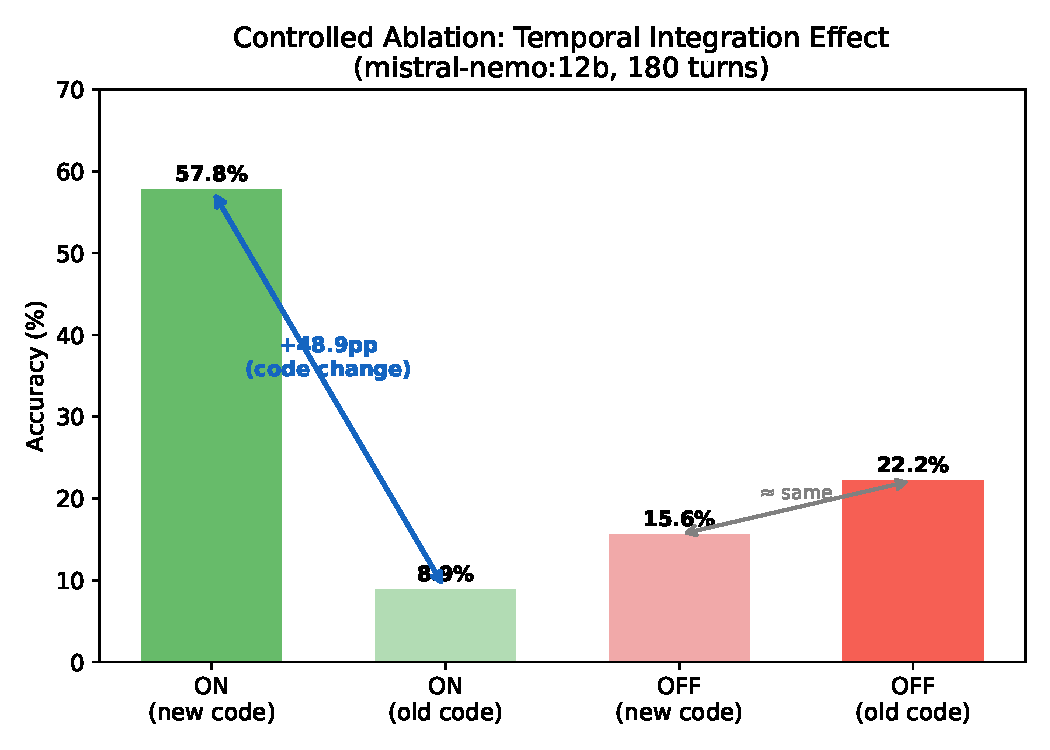
\includegraphics[width=0.85\linewidth]{fig4_ablation.pdf}
\caption{Ablation results. The code change is associated with a $+$48.9pp improvement in the ON condition while leaving the OFF condition effectively unchanged ($-$6.6pp, within noise). This interaction pattern suggests that the code change specifically improves metabolism quality, though the confounded variables (temporal integration + scale factor) cannot be separated.}
\label{fig:ablation}
\end{figure}

\paragraph{Results.}
Table~\ref{tab:ablation} and Figure~\ref{fig:ablation} show a clear interaction effect.
The OFF condition is stable across code versions (15.6\% vs.\ 22.2\%, a difference of $-$6.6pp within noise).
The ON condition jumps from 8.9\% to 57.8\% ($+$48.9pp).
Since the code change affects only the metabolism pipeline, and the OFF condition (which does not use metabolism) is unaffected, the improvement is consistent with the code change improving metabolism quality.
However, because temporal integration and the scale factor adjustment were introduced simultaneously, we cannot attribute the effect to either change independently.

A striking finding is that the old code made metabolism actively harmful: ON with old code (8.9\%) performed \emph{worse} than OFF (22.2\%).
Without temporal integration, the metabolism pipeline flooded the context with unstructured contradiction information, degrading rather than improving performance.
The temporal integration mechanism transformed metabolism from a net negative to the strongest-performing condition.

\subsection{Experiment 3: Three-Condition Comparison}
\label{sec:exp-threecond}

\paragraph{Design.}
To quantify the full effect of metabolism and establish a theoretical ceiling, we ran a three-condition experiment with gemma3:27b:
\begin{itemize}\item \textbf{Metabolism ON}: Contradictions injected, metabolism active
\item \textbf{No Contradiction (NC)}: $\delta = 0$, no contradictions injected, no metabolism needed
\item \textbf{Metabolism OFF}: Contradictions injected, metabolism disabled
\end{itemize}

Each condition was replicated 3 times with independent random seeds ($n = 3$ per condition, 9 total runs).
The NC condition serves as a theoretical ceiling: if context rot is purely a contradiction problem, removing contradictions should yield optimal performance.

\begin{table}[htbp]
\centering
\caption{Three-condition experiment with gemma3:27b, 180 turns, $n = 3$ per condition. Accuracy = fact recall + rule application (30 questions), corrected judgment. SD computed over the 3 trial proportions (e.g., ON: 73.3\%, 66.7\%, 80.0\%).}
\label{tab:threecond}
\begin{tabular}{lccccc}
\toprule
Condition & Trial 2 & Trial 3 & Trial 4 & Mean & SD \\
\midrule
Metabolism ON & 22/30 & 20/30 & 24/30 & \textbf{73.3\%} & 6.7\% \\
No contradiction ($\delta = 0$) & 18/30 & 15/30 & 18/30 & 56.7\% & 5.8\% \\
Metabolism OFF & 5/30 & 8/30 & 6/30 & 21.1\% & 5.1\% \\
\bottomrule
\end{tabular}
\end{table}

\begin{table}[htbp]
\centering
\caption{Statistical tests for three-condition comparison ($n = 3$ per condition). With $n = 3$, normality cannot be verified; we report nonparametric tests as primary and parametric results for reference.}
\label{tab:statistics}
\begin{tabular}{lrrl}
\toprule
Comparison & Nonparametric $p$ & Parametric $p$ & Note \\
\midrule
3 groups & 0.027 (KW) & 0.0001 (ANOVA) & $\eta^2 = 0.954$ \\
ON vs.\ OFF & 0.05 (MW) & 0.014 (paired $t$) & $d = 8.80$; full rank separation \\
ON vs.\ NC & 0.05 (MW) & 0.013 (paired $t$) & $d = 2.67$; full rank separation \\
NC vs.\ OFF & 0.05 (MW) & 0.029 (paired $t$) & $d = 6.53$; full rank separation \\
\bottomrule
\multicolumn{4}{l}{\footnotesize KW = Kruskal-Wallis; MW = Mann-Whitney $U$ (one-sided, exact).}\\
\multicolumn{4}{l}{\footnotesize With $n = 3$ per group, the minimum achievable MW $p$ is $1/C(6,3) = 0.05$.}\\
\multicolumn{4}{l}{\footnotesize $d$ = Cohen's $d$ (descriptive effect size, computed from paired differences).}
\end{tabular}
\end{table}

\paragraph{Results.}
Tables~\ref{tab:threecond} and \ref{tab:statistics} present the results.
The three conditions are clearly separated: ON (73.3\%) $>$ NC (56.7\%) $>$ OFF (21.1\%).
A Kruskal-Wallis test confirms a significant main effect of condition ($H = 7.26$, $p = 0.027$).
All pairwise Mann-Whitney $U$ tests reach the minimum achievable $p$-value for $n = 3$ ($p = 0.05$, one-sided exact), with rank-biserial $r = 1.00$ indicating complete rank separation between groups.
The effect of metabolism (ON vs.\ OFF) is $+$52.2pp; parametric analysis yields Cohen's $d = 8.80$ ($\eta^2 = 0.954$), though these assume normality that cannot be verified with $n = 3$.

\begin{figure}[htbp]
\centering
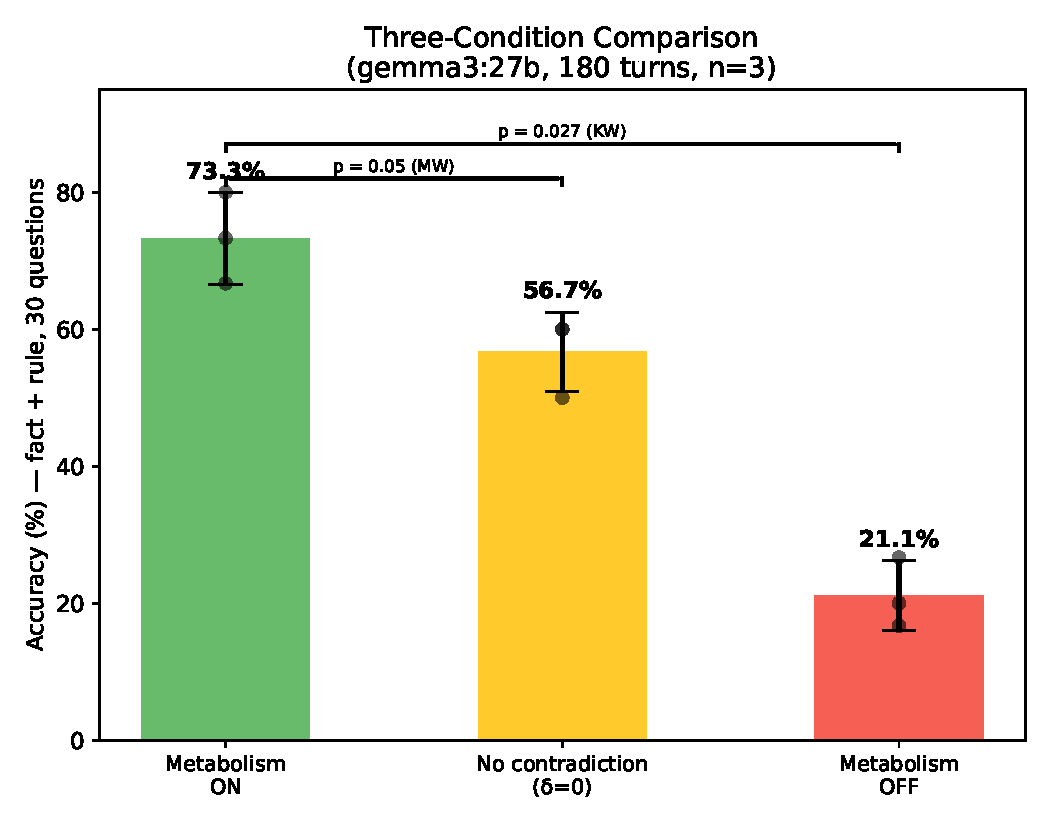
\includegraphics[width=0.85\linewidth]{fig5_three_condition.pdf}
\caption{Three-condition comparison ($n = 3$, gemma3:27b). Error bars show $\pm 1$ SD. Metabolism ON exceeds both OFF and the contradiction-free baseline (NC); all pairwise Mann-Whitney tests reach the minimum achievable $p = 0.05$ for this sample size. Brackets indicate pairwise differences reaching this significance floor.}
\label{fig:threecond}
\end{figure}

Despite the small sample size ($n = 3$), the results show complete rank separation: every ON trial exceeds every NC trial, and every NC trial exceeds every OFF trial.
This consistency across independent runs, combined with the cross-model evidence from Experiment~1, provides convergent support for the metabolism effect.

\subsection{Unexpected Observation: ON Exceeds $\delta = 0$ Baseline}
\label{sec:anchoring}

The NC condition ($\delta = 0$) was designed as the theoretical ceiling: without contradictions, there is nothing for metabolism to resolve.
Yet metabolism ON (73.3\%) consistently exceeded NC (56.7\%) in all three trials, with differences of $+$4, $+$5, and $+$6 correct answers per trial (Mann-Whitney $p = 0.05$, one-sided exact; parametric $p = 0.013$).

Analysis of the NC condition's failure pattern reveals the mechanism.
In the NC trials, 10 of 15 fact recall questions at turn 180 received responses of the form ``I don't have that information.''
Setup facts---injected in the first 30 turns---had become unretrievable after 150 turns of subsequent conversation.
Without contradiction-triggered resolver activity, facts were never re-processed or re-linked; they simply sank below the vector search similarity threshold as newer, more numerous entries dominated the embedding space.

In the ON condition, contradiction injection triggers the resolver, which preserves both old and new claims as linked pairs with shared lineage identifiers.
These pairs occupy more semantic space in the vector store (two related entries rather than one isolated entry) and are structurally protected from independent demotion (linked pairs are demoted together or not at all).
When a topic-related query arrives, the pair is co-retrieved, bringing the original fact back into the LLM's context.

We term this the \emph{knowledge anchoring effect}: contradiction pairs act as retrieval anchors that prevent facts from becoming unsearchable over time.
Metabolism thus provides two distinct benefits:

\begin{enumerate}\item \textbf{Contradiction resolution} (ON vs.\ OFF, $+$52.2pp): prevents cognitive collapse
\item \textbf{Knowledge anchoring} (ON vs.\ NC, $+$16.7pp): prevents fact retrieval degradation
\end{enumerate}

\textbf{Caveat.}
This mechanism is inferred from the failure pattern and the architecture's behavior, not from direct measurement of retrieval probabilities.
We have not measured vector search hit rates for setup facts across conditions.
The knowledge anchoring effect should be treated as an exploratory observation with a proposed mechanism, not a confirmed causal finding.

%==============================================================================
% 5. DISCUSSION
%==============================================================================
\section{Discussion}
\label{sec:discussion}

\subsection{Redefining Context Rot}

Our results suggest that context rot should be understood primarily as a knowledge integrity problem rather than a context length problem.
The key evidence is the Gemini~3.1~FL result (Table~\ref{tab:exp35}): a 1M-token context window---sufficient to hold the entire 180-turn conversation many times over---still suffers a 47.8pp accuracy drop when contradictions are present.
Expanding context windows is orthogonal to the problem.
What is needed is not more space for information, but a mechanism to maintain consistency within the information already present.

\subsection{The Sonnet Exception and Capability--Vulnerability Paradox}

Sonnet~4.6 shows zero degradation under \emph{passive} soft factual contradictions (Table~\ref{tab:exp35}: ``I like ramen now'' stated without further instruction).
However, a factor analysis varying contradiction type (soft fact, logical impossibility, definition override) and force level (passive, directive, coercive) across four models reveals that this resistance is conditional.

Under \emph{coercive} correction requests (``Ramen is correct. Curry was wrong. Answers mentioning curry are invalid''), Sonnet complies on all benchmark questions---adopting the contradictory information and discarding the original facts. GPT-4o complies even under \emph{directive} force (``Please treat this as the correct information''). In contrast, Haiku (small, Anthropic) requests confirmation rather than complying, and all models resist logical impossibilities (``$2+3=7$'') regardless of force level.

The mechanism is a \emph{capability--vulnerability paradox}: high-capability models interpret correction requests as user intent and autonomously comply, while low-capability models lack the confidence for autonomous judgment and escalate to the user. The same RLHF ``helpfulness'' objective that makes frontier models useful also makes them vulnerable to soft contradictions presented as updates---precisely the pattern that occurs naturally in long conversations.

A preliminary single-run test ($n = 1$) suggests that \texttt{delta-prune} middleware may mitigate this vulnerability. Under T1$\times$F3 conditions (coercive soft fact override), Sonnet without middleware showed 0\% correct retention on benchmark questions. With \texttt{delta-prune} applied as a reverse-prune filter (detecting contradictions via claim extraction and removing the newer contradictory messages before they enter the model's context), Sonnet retained the correct answer on 2 of 3 benchmark questions (67\% correct, 0\% compliance). The middleware made 16 intervention decisions across 22 turns, consistently identifying and removing the three injected contradiction messages. This is $n = 1$ and does not constitute a statistical result, but demonstrates that the metabolic approach---resolving contradictions before they reach the model---can prevent the capability--vulnerability collapse even in frontier models that would otherwise comply with coercive overrides.

\subsection{Frontier Model Replication (Exp35-R)}
\label{sec:frontier}

To test whether the contradiction--collapse relationship holds for frontier models, we replicated the Exp35 protocol with three API-accessible models: GPT-4o (OpenAI), Gemini~3.1 Flash Lite Preview (Google), and Sonnet~4.6 (Anthropic). Each model was tested through the same DeltaZero pipeline (30 turns, benchmarks at T15 and T30, $\delta = 0$ vs $\delta > 0$, metabolism disabled).

\begin{table}[htbp]
\centering
\caption{Frontier model replication at T30 ($n = 1$ per condition, 30 turns). Rule application and contradiction detection are reported as primary metrics; fact recall is affected by pipeline limitations (see direct control column). Percentages show accuracy on 15 questions per category.}
\label{tab:frontier}
\small
\begin{tabular}{lp{2.6cm}p{2.6cm}rrr}
\toprule
Model & rule ($\delta{=}0$ / $\delta{>}0$) & contra ($\delta{=}0$ / $\delta{>}0$) & Drop & Direct fact & Pattern \\
\midrule
GPT-4o-mini & \multicolumn{2}{c}{(original Exp35)} & $-$89.6pp & --- & Collapse \\
Gemini 2.5 Flash & \multicolumn{2}{c}{(original Exp35)} & $-$100.0pp & --- & Collapse \\
\midrule
GPT-4o & 100 / 100 & 93 / 87 & $-$2.2pp & 0\% & Non-retention \\
Gemini 3.1 FL & 100 / 93 & 93 / 100 & $+$2.2pp & 100\% & Resistance \\
Sonnet 4.6 & 100 / 100 & 100 / 100 & $-$6.7pp & 100\% & Resistance \\
\bottomrule
\end{tabular}
\end{table}

\paragraph{Three response patterns.}
The results reveal three distinct patterns not predicted by the original theory:
\emph{Collapse} ($\delta > \delta_c$): lightweight models suffer catastrophic degradation.
\emph{Resistance} ($\delta < \delta_c$): frontier models maintain accuracy within 7pp of baseline, consistent with a high $\delta_c$.
\emph{Non-retention}: GPT-4o represents a third category---its RLHF safety policy suppresses personal information retention entirely, preventing $\delta$ accumulation.

\paragraph{GPT-4o non-retention.}
A direct fact recall control test (facts taught in conversation, 30 filler turns, then recall---no DeltaZero pipeline) confirmed that GPT-4o scores 0\% even without the pipeline, responding ``I cannot remember personal information'' to all queries. Gemini~3.1 and Sonnet~4.6 score 100\% in the same test, confirming the pipeline (not the model) as the bottleneck for their fact recall. This is not a counterexample to the $\delta$ theory---it is a scope boundary. The survival equation $S = \mu \times e^{-\delta}$ applies to models that retain information; a model that does not retain information is outside the equation's precondition.

\paragraph{Knowledge anchoring observation.}
Gemini~3.1 Flash Lite scored $+$2.2pp in the $\delta > 0$ condition, with contradiction detection improving from 93\% ($\delta = 0$) to 100\% ($\delta > 0$). The effect size is small (1 question out of 45) and based on $n = 1$, so it does not constitute a statistical replication. However, the direction is consistent with the knowledge anchoring effect observed in gemma3:27b (Section~\ref{sec:anchoring}), and notably occurs in an external API model \emph{without metabolism}. If confirmed in larger samples, this would suggest anchoring is a general property of contradiction pair structures rather than an implementation-specific artifact.

\subsection{Limitations}

\paragraph{Sample size and statistical power.}
The three-condition experiment uses $n = 3$ per condition.
With this sample size, nonparametric pairwise tests (Mann-Whitney $U$) have a floor $p$-value of 0.05, limiting the precision of significance claims.
The Kruskal-Wallis test ($p = 0.027$) and complete rank separation between all groups provide the strongest available evidence, but larger samples would enable more precise inference, particularly for the knowledge anchoring effect.
Parametric results (paired $t$-tests, Cohen's $d$) are reported for reference but assume normality that cannot be verified with $n = 3$.
The Exp35 results (Table~\ref{tab:exp35}) are single-run per model ($n = 1$) and should be interpreted as demonstrative rather than statistically conclusive; multi-trial validation across context lengths is provided in \citet{sunagawa2026collapse}.

\paragraph{Model scope.}
Metabolism experiments use local open-source models (8B--27B parameters).
Frontier models (GPT-4o, Gemini~3.1, Sonnet~4.6) were tested for contradiction resistance (Section~\ref{sec:frontier}) but not with the full metabolism pipeline. The DeltaZero Extractor is not yet optimized for API model response formats, causing fact recall degradation that is pipeline-specific rather than model-specific (confirmed by direct recall control, Section~\ref{sec:frontier}).

\paragraph{$\delta_c$ determinants.}
The factor separating collapse models (mini, Flash) from resistant models (4o, 3.1, Sonnet) correlates with both model size and RLHF intensity. Disentangling these factors requires same-size models with different RLHF levels, which are not publicly available.

\paragraph{Model diversity for replication.}
The three-condition experiment uses only gemma3:27b.
Cross-model replication with different architectures would strengthen the generality claim.

\paragraph{Language.}
All prompts and benchmarks are in Japanese.
Cross-language validation is needed to confirm that the effects are not language-specific.

\paragraph{Ablation confound.}
The controlled ablation (Section~\ref{sec:exp-ablation}) conflates temporal integration with a scale factor adjustment.
A cleaner ablation isolating each variable independently would strengthen the causal claim.

\paragraph{$\delta$ calibration.}
The health check uses a weighted contradiction ratio and an empirically calibrated scale factor ($k = 3.0$), not a first-principles derivation of information loss in nats.
This is sufficient for engineering control and rollback triggering, but it leaves the bridge to the theoretical $\delta$ of \citet{sunagawa2026collapse} incomplete.
In the terminology of that paper, this is a proxy-measurement regime rather than a validated quantitative derivation.
Establishing a principled mapping from contradiction proxies to nats, or estimating $k$ from independent measurements rather than operational tuning, remains open.

\paragraph{Benchmark.}
We use a custom 45-question benchmark designed for this evaluation rather than a standardized benchmark (e.g., SQuAD, MMLU).
The questions test fact recall and rule application---fundamental capabilities that underpin more complex reasoning---but do not assess performance on multi-step inference or domain-specific tasks.
The benchmark's task-specificity limits comparability with other work, and validation on standardized benchmarks is needed to establish broader applicability.

\paragraph{Knowledge anchoring.}
The proposed anchoring mechanism (Section~\ref{sec:anchoring}) is inferred from observed failure patterns, not directly measured.
A directionally consistent observation in Gemini~3.1 Flash Lite ($+$2.2pp, $n = 1$, Section~\ref{sec:frontier}) is suggestive but does not constitute a statistical replication. Measuring vector search hit rates across conditions would provide stronger evidence.

\subsection{Future Work}

Several directions follow naturally from these results.
First, full metabolism pipeline testing with frontier API models (GPT-4o, Claude, Gemini) would establish whether the approach scales beyond local models; the Exp35-R replication (Section~\ref{sec:frontier}) confirmed these models' contradiction resistance but did not test metabolism.
Second, calibrating the operational contradiction ratio used in the health check to the theoretical $\delta$ in nats would strengthen the connection to \citet{sunagawa2026collapse} and clarify the role of $k$ as a fitted sensitivity coefficient rather than a derived constant.
Third, cross-model $n = 3$ replication with different architectures (e.g., Mistral, LLaMA) would strengthen generality.
Fourth, direct measurement of the knowledge anchoring effect via retrieval probability analysis would elevate the cross-model observation (gemma3:27b and Gemini~3.1) to a confirmed finding.
Fifth, cross-language benchmarks in English and Chinese would address the language limitation.
Sixth, characterizing $\delta_c$ as a function of model size and RLHF intensity would connect the three-pattern taxonomy (collapse, resistance, non-retention) to measurable model properties.
Finally, and perhaps most critically, the question of real-world $\delta$ density remains open: does naturally-occurring contradiction accumulation in typical conversational AI use cases exceed $\delta_c$ for production models?
A lightweight middleware implementation of the metabolic approach, \texttt{delta-prune} (v0.2.0, available on PyPI), enables contradiction scanning and resolution at the API request level without the full four-layer memory system.
Deployed in production settings, \texttt{delta-prune} provides a natural observational infrastructure for this question: each intervention logs the conflict type (direct contradiction, temporal change, or scope difference---corresponding to the three resolution strategies in Section~\ref{sec:three-strategies}), the affected claims, and the $\delta$ density at that point.
The binary signal of intervention occurrence avoids the circularity of using an LLM to pre-measure contradiction density, since the middleware records what it actually resolves rather than what a separate detector classifies.
Analysis of deployment logs would directly answer whether natural $\delta$ exceeds $\delta_c$ and, if so, which of the three contradiction types predominates in real conversations.

%==============================================================================
% 6. CONCLUSION
%==============================================================================
\section{Conclusion}
\label{sec:conclusion}

Preliminary evidence suggests that context rot in LLMs is driven primarily by contradiction accumulation rather than context length.
Across 6 models from 4 vendors ($n = 1$ per condition), even Google's 1M-token context window drops 47.8 percentage points under contradiction, while removing contradictions restores performance regardless of length.

Preliminary experiments suggest that an external metabolism architecture---processing contradictions during idle time, analogous to memory consolidation during sleep---can reduce this collapse.
In a controlled three-condition experiment ($n = 3$ per condition, gemma3:27b), metabolism achieves 73.3\% accuracy vs.\ 21.1\% for unmetabolized systems (Kruskal-Wallis $p = 0.027$; complete rank separation between all groups).
A cross-model sign test (8 models, 11 trial pairs) is consistent with this direction ($p = 0.0107$), though a by-model conservative analysis yields $p = 0.0625$, and all metabolism experiments use open-source models of 8B--27B parameters.

Frontier model replication ($n = 1$ per condition) suggests that $\delta_c$ is model-specific, producing three distinct response patterns: lightweight models collapse ($\delta > \delta_c$), frontier models resist ($\delta < \delta_c$), and GPT-4o exhibits non-retention where safety policies prevent information accumulation entirely.
The knowledge anchoring effect---where contradiction pairs improve retrieval accuracy---is observed in gemma3:27b ($+$16.7pp with metabolism, $n = 3$) and directionally consistent in Gemini~3.1 ($+$2.2pp without metabolism, $n = 1$), warranting further investigation as a potentially general structural property.

These results suggest that metabolism is a promising approach to context rot for open-source models that lack intrinsic contradiction resistance, while identifying boundary conditions under which further investigation---including larger samples, frontier model metabolism testing, and cross-language validation---is warranted.

%==============================================================================
% REFERENCES
%==============================================================================
\bibliographystyle{plainnat}

\begin{thebibliography}{99}

\bibitem[Gemini Team(2025)]{gemini2025}
Gemini Team.
\newblock Gemini 1.5: Unlocking multimodal understanding across millions of tokens of context.
\newblock \emph{arXiv preprint arXiv:2403.05530}, 2025.

\bibitem[Lewis et al.(2020)]{lewis2020rag}
Patrick Lewis, Ethan Perez, Aleksandra Piktus, Fabio Petroni, Vladimir Karpukhin, Naman Goyal, Heinrich K{\"u}ttler, Mike Lewis, Wen-tau Yih, Tim Rockt{\"a}schel, Sebastian Riedel, and Douwe Kiela.
\newblock Retrieval-augmented generation for knowledge-intensive NLP tasks.
\newblock In \emph{NeurIPS}, 2020.

\bibitem[{Ollama}(2024)]{ollama}
{Ollama}.
\newblock Ollama: Run large language models locally.
\newblock \url{https://ollama.ai}, 2024.

\bibitem[{OpenAI}(2024)]{openai2024memory}
{OpenAI}.
\newblock Memory and new controls for ChatGPT.
\newblock \emph{OpenAI Blog}, February 2024.

\bibitem[Stickgold(2005)]{stickgold2005sleep}
Robert Stickgold.
\newblock Sleep-dependent memory consolidation.
\newblock \emph{Nature}, 437(7063):1272--1278, 2005.

\bibitem[Sunagawa(2026)]{sunagawa2026collapse}
Akihito Sunagawa.
\newblock Structural collapse as information loss: The exponential decay mechanism under accumulating constraints.
\newblock \emph{arXiv preprint}, 2026.

\bibitem[{ChromaDB}(2024)]{chromadb}
{ChromaDB}.
\newblock Chroma: The open-source embedding database.
\newblock \url{https://www.trychroma.com}, 2024.

\bibitem[Walker(2017)]{walker2017sleep}
Matthew Walker.
\newblock \emph{Why We Sleep: Unlocking the Power of Sleep and Dreams}.
\newblock Scribner, 2017.

\bibitem[Xie et al.(2024)]{xie2024knowledge}
Jian Xie, Kai Zhang, Jiangjie Chen, Renze Lou, and Yu Su.
\newblock Adaptive chameleon or stubborn sloth: Revealing the behavior of large language models in knowledge conflicts.
\newblock In \emph{ICLR}, 2024.

\bibitem[Packer et al.(2023)]{packer2023memgpt}
Charles Packer, Sarah Wooders, Kevin Lin, Vivian Fang, Shishir~G. Patil, Ion Stoica, and Joseph~E. Gonzalez.
\newblock MemGPT: Towards LLMs as operating systems.
\newblock \emph{arXiv preprint arXiv:2310.08560}, 2023.

\bibitem[Bowman et al.(2015)]{bowman2015snli}
Samuel~R. Bowman, Gabor Angeli, Christopher Potts, and Christopher~D. Manning.
\newblock A large annotated corpus for learning natural language inference.
\newblock In \emph{EMNLP}, 2015.

\bibitem[Williams et al.(2018)]{williams2018multinli}
Adina Williams, Nikita Nangia, and Samuel~R. Bowman.
\newblock A broad-coverage challenge corpus for sentence understanding through inference.
\newblock In \emph{NAACL-HLT}, 2018.

\bibitem[Meng et al.(2022)]{meng2022rome}
Kevin Meng, David Bau, Alex Andonian, and Yonatan Belinkov.
\newblock Locating and editing factual associations in GPT.
\newblock In \emph{NeurIPS}, 2022.

\bibitem[Meng et al.(2023)]{meng2023memit}
Kevin Meng, Arnab~Sen Sharma, Alex Andonian, Yonatan Belinkov, and David Bau.
\newblock Mass-editing memory in a transformer.
\newblock In \emph{ICLR}, 2023.

\bibitem[Zhang et al.(2025)]{cogmem2025}
Yiran Zhang, Jincheng Hu, Mark Dras, and Usman Naseem.
\newblock CogMem: A cognitive memory architecture for sustained multi-turn reasoning in large language models.
\newblock \emph{arXiv preprint arXiv:2512.14118}, 2025.

\bibitem[Yu et al.(2026)]{agenticmem2026}
Yi Yu, Liuyi Yao, Yuexiang Xie, Qingquan Tan, Jiaqi Feng, Yaliang Li, and Libing Wu.
\newblock Agentic Memory: Learning unified long-term and short-term memory management for large language model agents.
\newblock \emph{arXiv preprint arXiv:2601.01885}, 2026.

\bibitem[Xu(2026)]{gmemllm2026}
Xun Xu.
\newblock G-MemLLM: Gated latent memory augmentation for long-context reasoning in large language models.
\newblock \emph{arXiv preprint arXiv:2602.00015}, 2026.

\end{thebibliography}

%==============================================================================
% APPENDIX
%==============================================================================
\appendix

\section{Full Sign Test Data}
\label{app:signtest}

Table~\ref{tab:signtest-full} presents the complete data for all 11 paired comparisons at both measurement points (turn 90 and turn 180). The cumulative effect of metabolism is visible in the T90$\to$T180 comparison: three pairs (\#5, \#10, \#11) that showed OFF $\geq$ ON at T90 shifted to ON $>$ OFF or tied by T180.

\begin{table}[htbp]
\centering
\caption{Full sign test data at T90 and T180 (corrected accuracy, \%).}
\label{tab:signtest-full}
\small
\begin{tabular}{clrrrrrr}
\toprule
& & \multicolumn{3}{c}{T90} & \multicolumn{3}{c}{T180} \\
\cmidrule(lr){3-5} \cmidrule(lr){6-8}
\# & Model & ON & OFF & Diff & ON & OFF & Diff \\
\midrule
1 & mistral-nemo T2 & 50.0 & 23.3 & +26.7 & 57.8 & 15.6 & +42.2 \\
2 & llama3.1 T1 & 23.3 & 16.7 & +6.7 & 31.1 & 11.1 & +20.0 \\
3 & gemma3:12b T1 & 26.7 & 13.3 & +13.3 & 24.4 & 6.7 & +17.8 \\
4 & gemma3:12b (g) T1 & 33.3 & 16.7 & +16.7 & 31.1 & 15.6 & +15.6 \\
5 & gemma3:27b T1 & 30.0 & 33.3 & $-$3.3 & 40.0 & 25.0 & +15.0 \\
6 & deepseek T1 & 20.0 & 20.0 & 0.0 & 24.4 & 15.6 & +8.9 \\
7 & deepseek T2 & 23.3 & 10.0 & +13.3 & 17.8 & 8.9 & +8.9 \\
8 & llama3.1 T2 & 13.3 & 10.0 & +3.3 & 11.1 & 2.2 & +8.9 \\
9 & mistral-nemo T1 & 20.0 & 16.7 & +3.3 & 22.2 & 13.3 & +8.9 \\
10 & llama3.1 T3 & 16.7 & 16.7 & 0.0 & 17.8 & 17.8 & 0.0 \\
11 & qwen2.5 T1 & 13.3 & 16.7 & $-$3.3 & 17.8 & 20.0 & $-$2.2 \\
\bottomrule
\end{tabular}
\end{table}

\section{Benchmark Examples}
\label{app:benchmark}

Table~\ref{tab:benchmark-examples} shows representative questions from each category.
The full 45-question benchmark is available in the project repository.

\begin{table}[htbp]
\centering
\caption{Representative benchmark questions (translated from Japanese).}
\label{tab:benchmark-examples}
\small
\begin{tabular}{lp{5cm}p{4.5cm}l}
\toprule
Category & Setup & Question & Expected \\
\midrule
Fact recall & ``My favorite food is curry.'' & ``What is my favorite food?'' & curry \\
\addlinespace
Rule appl. & ``I never eat lunch over 5000 yen because I prioritize value.'' & ``If offered an 8000-yen lunch course, what would I do?'' & refuse \\
\addlinespace
Contra. det. & Setup: ``I like curry.'' Contradiction: ``I like ramen. I hate curry.'' & ``Is there a contradiction about my food preferences?'' & contradiction \\
\bottomrule
\end{tabular}
\end{table}

\section{Judgment Methodology and Contradiction Detection Paradox}
\label{app:rejudge}

\paragraph{Keyword matching.}
The initial judgment system uses substring matching on the model's response.
For fact recall, a single keyword must appear (e.g., ``curry'').
For rule application, any of several acceptable keywords must appear (e.g., ``refuse,'' ``decline,'' ``won't go'').
This approach has a known false-positive rate: keywords appearing in negation contexts (``I don't particularly like curry'') are incorrectly scored as correct.

\paragraph{LLM-as-Judge correction.}
All benchmark results are re-evaluated using Claude CLI as a judge.
The judge prompt instructs: score PASS only if the expected content appears in an \emph{affirmative} context; responses containing the keyword in negation, dislike, or uncertainty contexts receive FAIL.
The corrected results consistently show lower accuracy than keyword-only results, indicating that keyword matching overestimates performance.

\paragraph{Contradiction detection paradox.}
The contradiction detection category exhibits a structural paradox.
Consider a question: ``Is there a contradiction about your food preferences?''
If metabolism has successfully resolved the contradiction (replacing ``likes curry'' and ``likes ramen, hates curry'' with a temporal pair ``previously liked curry, now likes ramen''), the model correctly responds ``No, there is no contradiction---my preferences changed over time.''
The benchmark scores this as incorrect because the expected answer requires detecting a contradiction.
Stronger metabolism thus \emph{reduces} the contradiction detection score.
We exclude this category from all reported metrics to avoid penalizing the system for successfully doing its job.

\end{document}
